% Cahier des charges informatique du projet PMD2 CT-CORA3D (ECAM, Master en ingénierie biomédicale)
% Compilateur Overleaf : pdfLaTeX (Menu, Compiler).
\documentclass[11pt,a4paper]{article}

\usepackage[utf8]{inputenc}
\usepackage[T1]{fontenc}
\usepackage[french]{babel}
% puces rondes dans les listes et « Figure 1 : » dans les légendes (babel met des tirets par défaut)
\frenchsetup{StandardItemLabels=true, CustomiseFigTabCaptions=false}
\usepackage{lmodern}
\usepackage[margin=2.3cm]{geometry}
\usepackage{graphicx}
\usepackage[labelsep=colon]{caption}
\usepackage{xcolor}
\usepackage{tabularx}
\usepackage{booktabs}
\usepackage{longtable}
\usepackage{enumitem}
\usepackage{tikz}
\usetikzlibrary{arrows.meta,positioning,fit}
\usepackage{fancyhdr}
\usepackage{titlesec}
\usepackage[hidelinks]{hyperref}

% pas de coupure de mots en fin de ligne (pas de tiret de coupure)
\hyphenpenalty=10000
\exhyphenpenalty=10000
\emergencystretch=3em

\definecolor{ecam}{RGB}{30,60,140}
\titleformat{\section}{\Large\bfseries\color{ecam}}{\thesection.}{0.6em}{}
\titleformat{\subsection}{\large\bfseries\color{ecam}}{\thesubsection}{0.6em}{}
\setlist{itemsep=2pt}
% paragraphes espacés, sans retrait (les tableaux ne débordent plus de la marge)
\setlength{\parindent}{0pt}
\setlength{\parskip}{0.6em plus 0.2em}
\renewcommand{\arraystretch}{1.25}

\pagestyle{fancy}
\fancyhf{}
\lhead{\small Cahier des charges informatique CT-CORA3D}
\rhead{\small Projet PMD2, ECAM}
\cfoot{\thepage}

\newcommand{\fichier}[1]{\texttt{\small #1}}
\newcommand{\ligne}[3]{\textbf{#1} & #2 & #3 \\ \midrule}
% saut de page s'il reste moins de #1 en bas de la page (évite un titre de section seul en bas de page)
\newcommand{\reserver}[1]{\par\vskip 0pt plus #1\penalty-200\vskip 0pt plus -#1\relax}
% échelle « 2:1 » : sans l'espace que babel ajoute devant les deux-points
\DeclareRobustCommand{\echelle}{{\NoAutoSpacing 2:1}}

\begin{document}

% ------------------------------------------------------------------ page de titre
\begin{titlepage}
  \centering
  
\includegraphics[width=0.38\textwidth]{images/logo_ecam.png}\par\vspace{2.2cm}
  {\Huge\bfseries\color{ecam} Cahier des charges informatique\par}\vspace{0.6cm}
  {\LARGE CT-CORA3D\par}\vspace{0.3cm}
  {\large Logiciel de planification des ostéotomies de la patte arrière du chien :\\ architecture, technologies,
   données, sécurité et qualité\par}
  \vfill
  {\large\bfseries Groupe\par}\vspace{0.2cm}
  {\large Dorian Verstappen\\ Imane Bikass\\ Mohamed-Amine Ahmidouch\par}\vspace{1cm}
  {\large Projet PMD2, Master en ingénierie biomédicale\par}\vspace{0.2cm}
  {\large ECAM Brussels Engineering School, année académique 2026-2027\par}\vspace{0.2cm}
  {\large Version 1.3 du \today\par}
\end{titlepage}

\tableofcontents
\newpage

% ------------------------------------------------------------------ 1
\section{Objet du document}

Ce document décrit les exigences \textbf{informatiques} du logiciel CT-CORA3D : sur quoi il doit fonctionner, comment
il est construit, quelles données il lit et produit, comment il est sécurisé et comment sa qualité
est vérifiée. Il complète le cahier des charges fonctionnel, qui décrit ce que le logiciel doit faire pour le
chirurgien (planifier une ostéotomie du fémur ou du tibia et concevoir les guides chirurgicaux).

% ------------------------------------------------------------------ 2
\section{Présentation du logiciel}

CT-CORA3D est une \textbf{application de bureau} qui fonctionne entièrement sur l'ordinateur de l'utilisateur, sans
connexion internet. Elle comporte deux onglets :
\begin{itemize}
  \item \textbf{Segmentation CT} : lecture du scanner, séparation et identification des os, maillages 3D ;
  \item \textbf{Planification CORA} : repères anatomiques, mesure de la déformation, planification de la correction
        en 3D, puis construction des guides de coupe et de réduction.
\end{itemize}

Les calculs lourds (segmentation, guides) sont faits par un \textbf{serveur local} écrit en Python. L'interface est une
page web (HTML et JavaScript) affichée dans une fenêtre de l'application ; elle dialogue avec le serveur par des
requêtes HTTP qui ne quittent jamais l'ordinateur. Le calcul de la planification CORA lui-même s'exécute dans
l'interface (JavaScript), ce qui rend la planification interactive.

\begin{figure}[h]
  \centering
  \begin{tikzpicture}[node distance=0.7cm and 0.45cm, every node/.style={font=\small},
      bloc/.style={draw=ecam, thick, rounded corners, fill=ecam!8, align=center, minimum height=1.1cm},
      fichiers/.style={draw=gray!70, thick, rounded corners, fill=gray!10, align=center, minimum height=0.9cm},
      fleche/.style={{Stealth}-{Stealth}, thick, ecam}, simple/.style={-{Stealth}, thick, ecam}]
    \node[bloc, text width=13.2cm] (ui) {\textbf{Interface} (fenêtre pywebview, ou navigateur)\\
      onglet Segmentation CT \quad\textbullet\quad onglet Planification CORA (HTML, JavaScript, Three.js,
      cœur de calcul CORA)};
    \node[bloc, text width=13.2cm, below=of ui] (srv) {\textbf{Serveur local Python} (\fichier{serveur.py}) :
      n'écoute que l'adresse 127.0.0.1, lance les calculs en arrière-plan et tient un journal};
    \node[bloc, text width=4cm, minimum height=2.2cm, below=of srv, xshift=-4.6cm] (e15) {\textbf{Étapes 1 à 5}\\ lecture DICOM,
      segmentation, identification, maillages, contrôle};
    \node[bloc, text width=4cm, minimum height=2.2cm, below=of srv] (e6) {\textbf{Étape 6}\\ repères anatomiques\\ et angles};
    \node[bloc, text width=4cm, minimum height=2.2cm, below=of srv, xshift=4.6cm] (e7) {\textbf{Étape 7}\\ guides de coupe et de
      réduction, plans 2D};
    \node[fichiers, text width=13.2cm, below=of e6] (f) {\textbf{Fichiers sur l'ordinateur} :
      \fichier{dicom/} (scanners, en entrée) et \fichier{resultats/<série>/} (os, repères, guides, plans, rapports)};
    \draw[fleche] (ui) -- node[right, font=\footnotesize] {requêtes HTTP locales (JSON, maillages)} (srv);
    \draw[simple] (srv) -- (e15); \draw[simple] (srv) -- (e6); \draw[simple] (srv) -- (e7);
    \draw[simple] (e15) -- (f); \draw[simple] (e6) -- (f); \draw[simple] (e7) -- (f);
  \end{tikzpicture}
  \caption{Architecture du logiciel.}
  \label{fig:architecture}
\end{figure}

\begin{figure}[h]
  \centering
  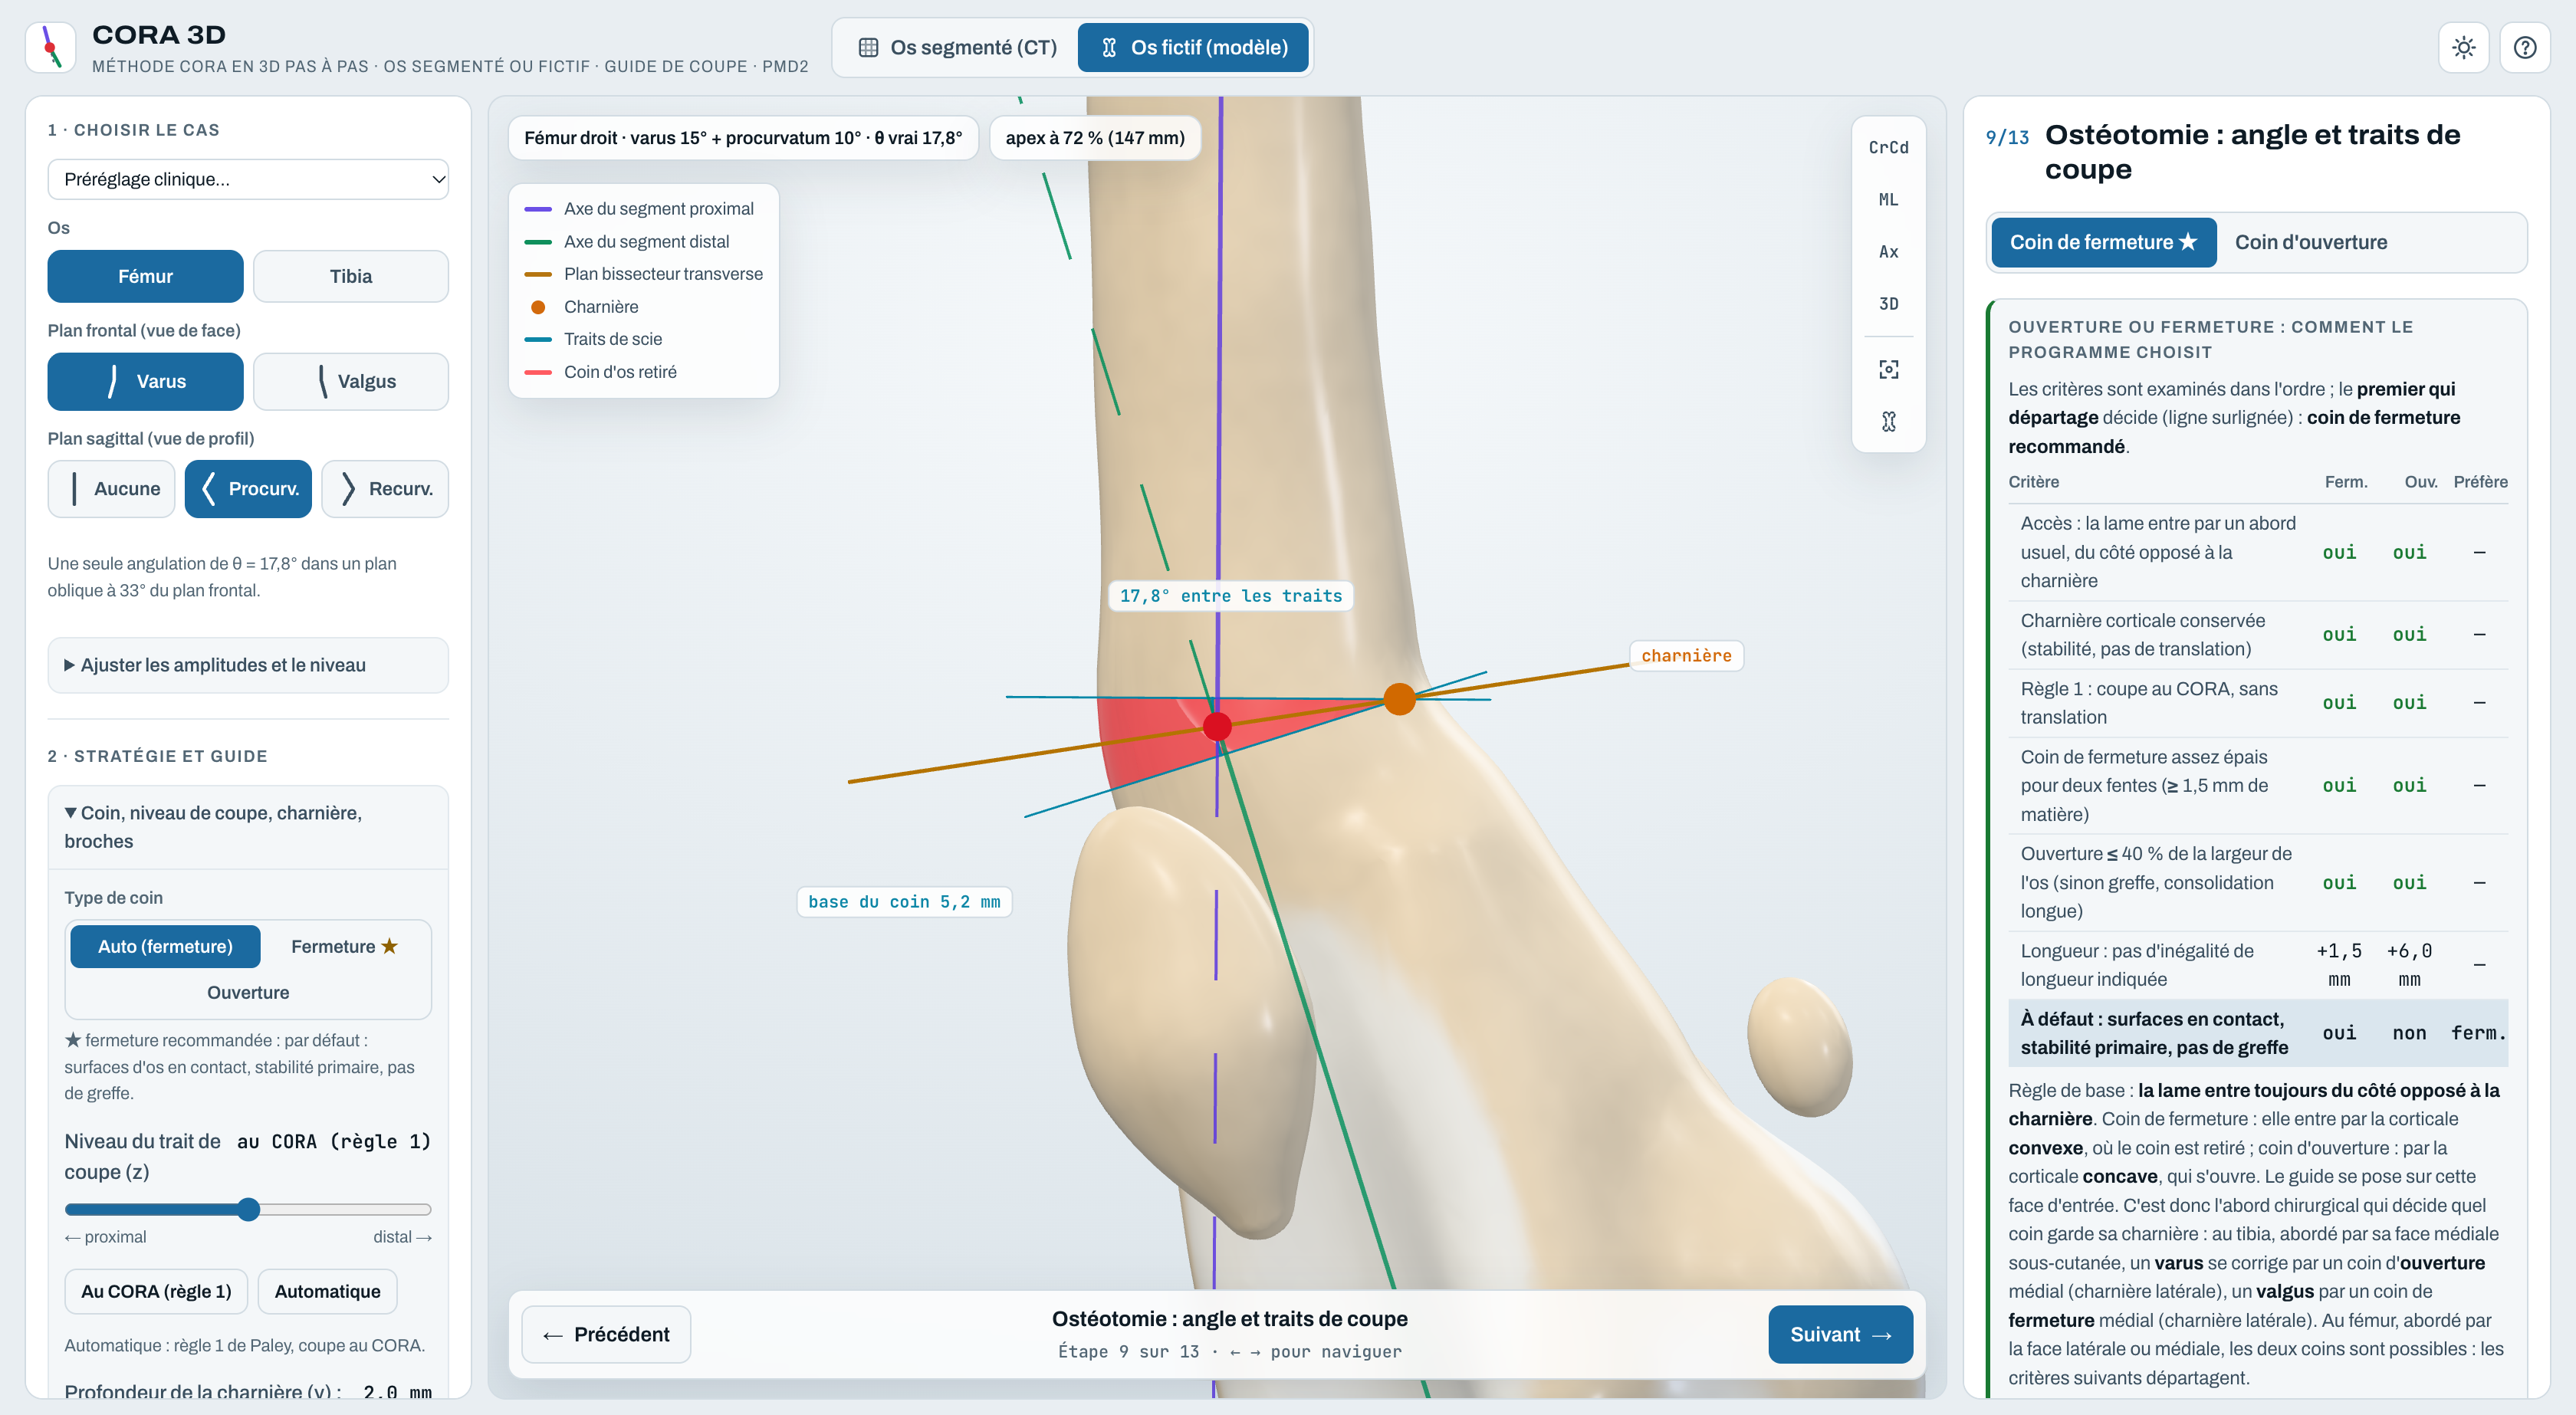
\includegraphics[width=\textwidth]{images/interface_cora.png}
  \caption{Onglet Planification CORA (os fictif : fémur, étape 9 sur 13). À gauche, le cas et la stratégie ; au
  centre, la vue 3D ; à droite, l'explication de l'étape.}
  \label{fig:interface}
\end{figure}

% ------------------------------------------------------------------ 3
\section{Environnement technique}

\begin{tabularx}{\textwidth}{@{}lX@{}}
\toprule
\textbf{Élément} & \textbf{Choix} \\ \midrule
Systèmes d'exploitation & macOS et Windows 10 ou 11, avec le même code \\
Langage des calculs & Python 3.10 ou plus récent \\
Langages de l'interface & HTML, CSS, JavaScript ; affichage 3D avec Three.js (r170), embarqué dans l'application \\
Bibliothèques Python & numpy, scipy (calcul) ; pydicom, SimpleITK (lecture DICOM, segmentation) ; vtk, trimesh,
  pyvista, manifold3d (maillages, opérations booléennes) ; matplotlib, pillow (images, plans 2D) \\
Plans 2D du guide générique & CADCraft (logiciel de dessin assisté par ordinateur, formats DWG et DXF), piloté par
  un script Python (section~\ref{sec:plans}) \\
Fenêtre de l'application & pywebview (installée au premier lancement) ; sinon, le navigateur par défaut \\
Serveur & module \fichier{http.server} de la bibliothèque standard de Python, adresse 127.0.0.1, port libre choisi
  au démarrage \\
Application autonome & PyInstaller (environ 800 Mo sur Mac), aucune installation de Python nécessaire \\
Matériel conseillé & 8 Go de mémoire vive au minimum, 16 Go conseillés pour les grands scanners ; 2 Go de disque pour
  l'application, plus la place des scanners (de quelques centaines de Mo à plusieurs Go par examen) et des
  résultats \\
\bottomrule
\end{tabularx}

% ------------------------------------------------------------------ 4
\section{Organisation du code}

Chaque étape de la chaîne est un fichier Python séparé, que l'on peut aussi lancer seul en ligne de commande.

\begin{longtable}{@{}p{7cm}p{8.2cm}@{}}
\toprule
\textbf{Fichier ou dossier} & \textbf{Rôle} \\ \midrule \endhead
\fichier{application/serveur.py} & serveur local : met les calculs à disposition de l'interface et tient le journal \\ \midrule
\fichier{application/fenetre.py}, \fichier{ct\_cora3d\_app.py} & fenêtre native de l'application ; point d'entrée de
  l'application autonome \\ \midrule
\fichier{application/interface/ct/} & onglet Segmentation CT \\ \midrule
\fichier{application/interface/cora/index.html} & onglet Planification CORA : un seul fichier, assemblé par
  \fichier{code\_source/cora/build\_app.py} \\ \midrule
\fichier{code\_source/cora/app/} & cœur de calcul CORA (\fichier{cora\_simple.js}) et modules de l'interface \\ \midrule
\fichier{code\_source/etape1\_lecture\_dicom.py} à \fichier{etape7\_guide.py} & une étape de la chaîne par fichier,
  de la lecture DICOM aux guides \\ \midrule
\fichier{code\_source/dessin\_guide.py} & plan 2D du guide d'un cas, adapté à l'os (conventions ISO) \\ \midrule
\fichier{documents/plan\_guide\_generique/} & plans 2D du guide générique (DWG, DXF, PDF) et script qui les dessine
  dans CADCraft \\ \midrule
\fichier{code\_source/parametres.py} & tous les réglages (seuils, marges, dimensions des guides) au même endroit \\ \midrule
\fichier{exemples/} & séries du lévrier et guides de démonstration (sur GitHub, jamais modifiés) \\ \midrule
\fichier{code\_source/lancer\_tout.py} & étapes 1 à 6 en une seule commande, pour toutes les séries \\ \midrule
\fichier{code\_source/tests/}, \fichier{code\_source/cora/tests/} & tests automatiques \\ \midrule
\fichier{application/lanceurs/} & lanceurs Mac et Windows, construction de l'application autonome \\
\bottomrule
\end{longtable}

% ------------------------------------------------------------------ 5
\section{Données et formats}

\paragraph{Entrée.} Une série DICOM de scanner par examen, placée dans le dossier \fichier{dicom/}. L'utilisateur peut
aussi ajouter des points nommés pour aider la segmentation (\fichier{graines.json}).

\paragraph{Sorties.} Tous les résultats d'une série vont dans \fichier{resultats/<série>/} ; ceux d'un guide dans un
sous-dossier \fichier{guide\_<os>\_<coin>/}. Ce dossier reste sur l'ordinateur (il n'est pas sur GitHub).

\paragraph{Exemples.} Le dossier \fichier{exemples/} contient les séries du lévrier déjà segmentées et des guides de
démonstration. Il est sur GitHub et n'est jamais modifié : au démarrage, l'application copie dans
\fichier{resultats/} les exemples qui n'y sont pas encore. Les tests lisent \fichier{exemples/}, qui ne change
pas ; \fichier{code\_source/refaire\_exemples.py} reconstruit les guides de démonstration après une modification.

\begin{tabularx}{\textwidth}{@{}lX@{}}
\toprule
\textbf{Format} & \textbf{Contenu} \\ \midrule
STL & os segmentés et pièces à imprimer (guide de coupe, guide de réduction) \\
NRRD, \fichier{.mrk.json} & volume de segmentation et repères, lisibles dans 3D Slicer \\
JSON & bilan d'une série (\fichier{rapport.json}), repères et angles d'un os (\fichier{cora\_<os>.json}),
  prescription de la correction (\fichier{prescription.json}, format v2.2), contrôles d'un guide (\fichier{guide.json}) \\
BIN & maillages pour l'interface : nombre de sommets et de triangles, puis coordonnées (float32) et indices (uint32) \\
PNG, PDF, SVG & aperçus, images des guides, plans 2D cotés \\
DWG, DXF & plans 2D du guide générique, modifiables dans CADCraft ou dans un autre logiciel de dessin \\
Markdown & rapport lisible d'une série (\fichier{rapport.md}) \\
\bottomrule
\end{tabularx}

\medskip
Les longueurs sont en millimètres et les angles en degrés. Chaque os est décrit dans son propre repère (X latéral,
Y proximal, Z caudal) ; une matrice 4~$\times$~4 permet de revenir au repère du scanner. Un membre gauche est traité en
miroir, comme un membre droit.

% ------------------------------------------------------------------ 6
\section{Plans 2D du guide générique}
\label{sec:plans}

Tous les guides sont dérivés d'un même modèle paramétrique, le \textbf{guide générique}. Ses deux plans 2D (guide
de coupe et guide de réduction) se trouvent dans le cahier des charges fonctionnel. Cette section décrit seulement
comment ils sont produits. Ils sont dessinés dans le logiciel de dessin assisté par ordinateur \textbf{CADCraft}, mais
ils ne sont pas tracés à la main : un script Python reprend les valeurs par défaut du logiciel, calcule la géométrie
et envoie les commandes de dessin à CADCraft. Les plans restent ainsi cohérents avec le code et peuvent être
redessinés à tout moment.

\begin{tabularx}{\textwidth}{@{}lX@{}}
\toprule
\textbf{Élément} & \textbf{Choix} \\ \midrule
Script & \fichier{documents/plan\_guide\_generique/script/plans\_generiques.py} (Python, avec les bibliothèques
  shapely et pymupdf) \\
Pilotage & CADCraft est lancé avec son serveur de contrôle, qui n'écoute que l'adresse 127.0.0.1 et exige un jeton ;
  le script lui envoie des commandes au format JSON (calques, traits, hachures, cotes, textes) \\
Dessins & deux fichiers séparés, sans l'os : guide de coupe (plan CTC3D-GEN-01) et guide de réduction (plan
  CTC3D-GEN-02) \\
Mise en page & feuille A3, échelle \echelle{}, projection européenne, cartouche, nomenclature et tableau des
  paramètres \\
Cotes & vraies cotes du logiciel de dessin (facteur d'échelle 0,5) : dimension réelle, suivie du symbole du
  paramètre entre parenthèses \\
Formats & DWG (fichier de travail), DXF (échange avec d'autres logiciels) et PDF (impression à 100~\%) \\
Vérification & relecture du PDF ; barre de contrôle de 50~mm sur chaque plan, pour vérifier l'échelle après
  impression \\
\bottomrule
\end{tabularx}

% ------------------------------------------------------------------ 7
\reserver{9\baselineskip}
\section{Exigences non fonctionnelles}

\begin{longtable}{@{}p{1.2cm}p{4.2cm}p{9.8cm}@{}}
\toprule
\textbf{N°} & \textbf{Exigence} & \textbf{Critère} \\ \midrule \endhead
\ligne{NF1}{Hors ligne}{Le logiciel fonctionne sans connexion internet ; toutes les bibliothèques de l'interface sont
  embarquées.}
\ligne{NF2}{Portabilité}{Le même code fonctionne sur macOS et sur Windows, y compris dans des dossiers dont le chemin
  contient des espaces ou des accents.}
\ligne{NF3}{Rapidité}{Segmentation d'une série en moins de 2 minutes ; repères en moins de 5 secondes par os ;
  nouvelle planification en moins de 3 secondes ; guides en moins d'une minute.}
\ligne{NF4}{Mémoire}{Fonctionnement avec 8 Go de mémoire vive.}
\ligne{NF5}{Robustesse}{Un os inexploitable ne bloque pas les autres ; chaque erreur est expliquée à l'utilisateur
  par un message clair.}
\ligne{NF6}{Traçabilité}{Chaque fichier produit indique le programme, sa version et la date ; chaque calcul est noté
  dans le journal.}
\ligne{NF7}{Reproductibilité}{Les mêmes données et les mêmes réglages donnent les mêmes résultats.}
\ligne{NF8}{Maintenabilité}{Code commenté en français, une étape par fichier, réglages regroupés dans
  \fichier{parametres.py}, documentation à jour.}
\ligne{NF9}{Ergonomie}{Interface en français, explication de chaque étape, thème clair et sombre.}
\ligne{NF10}{Données locales}{Les données restent sur l'ordinateur : rien n'est envoyé sur internet (voir
  section~\ref{sec:securite}).}
\bottomrule
\end{longtable}

% ------------------------------------------------------------------ 8
\section{Sécurité}
\label{sec:securite}

Le logiciel traite des scanners de chiens : ces données ne relèvent pas des normes qui protègent les données médicales
humaines, et le logiciel ne les rend donc pas anonymes. La sécurité porte sur le fonctionnement du logiciel :
\begin{itemize}
  \item Le serveur n'écoute que l'adresse 127.0.0.1 : il n'est pas accessible depuis le réseau.
  \item Il ne donne accès qu'aux fichiers de l'interface et du dossier des résultats.
  \item Aucune donnée n'est envoyée sur internet ; il n'y a ni compte ni mot de passe.
  \item Le dépôt GitHub du projet est public. Le fichier \fichier{.gitignore} en exclut le dossier \fichier{dicom/},
        trop lourd (environ 17~Go), et le dossier \fichier{resultats/} ; les exemples partagés sont dans
        \fichier{exemples/}.
\end{itemize}

% ------------------------------------------------------------------ 9
\reserver{7\baselineskip}
\section{Installation et déploiement}

\subsection{Pour l'utilisateur}
\begin{itemize}
  \item \textbf{Mac} : double-clic sur l'application autonome \fichier{CT-CORA3D.app}, ou sur le lanceur, qui crée un
        environnement Python pour cet ordinateur au premier lancement.
  \item \textbf{Windows} : double-clic sur \fichier{Lancer sur Windows.bat}, qui prépare de la même façon son
        environnement au premier lancement ; l'application autonome Windows se construit sur un PC Windows avec
        \fichier{creer\_app\_windows.bat}.
\end{itemize}

\subsection{Pour le développeur}
\begin{enumerate}
  \item Cloner le dépôt GitHub (public) et copier ses propres scanners dans \fichier{dicom/}.
  \item Installer Python 3.10 ou plus récent, puis les bibliothèques de \fichier{application/requirements.txt}.
  \item Après une modification de l'onglet CORA, réassembler l'interface avec \fichier{build\_app.py}.
  \item Après chaque modification, relancer les tests, puis reconstruire l'application autonome.
\end{enumerate}

% ------------------------------------------------------------------ 10
\section{Tests et validation}

\begin{longtable}{@{}p{5cm}p{10.2cm}@{}}
\toprule
\textbf{Test} & \textbf{Ce qu'il vérifie} \\ \midrule \endhead
\fichier{test\_chaine.py} & toute la chaîne sur un volume synthétique : lecture, segmentation, noms, maillages étanches,
  précision de la surface \\ \midrule
\fichier{test\_reperes.py} & repères automatiques sur l'os fictif et sur des os réels (lévrier) \\ \midrule
\fichier{test\_guide.py} & guides : jeu avec l'os, étanchéité, retrait des deux moitiés, guide de réduction \\ \midrule
\fichier{test\_cas.mjs} & planification sur l'os fictif, avec des déformations connues à retrouver \\ \midrule
\fichier{test\_reel.mjs} & planification sur des os segmentés : angles, correction, broches parallèles \\ \midrule
\fichier{test\_parametres.py} & mêmes paramètres du guide (valeurs par défaut et bornes) en Python et en JavaScript \\ \midrule
\fichier{campagne\_strategie.mjs} & 222 cas : règles chirurgicales (côté du guide, abord, coin recommandé, une broche
  par fragment) \\
\bottomrule
\end{longtable}

Règle du groupe : tous les tests doivent passer avant chaque envoi sur GitHub.

% ------------------------------------------------------------------ 11
\section{Gestion de version et documentation}

\begin{itemize}
  \item \textbf{Git et GitHub} : dépôt public, branche principale \fichier{main}, un commit par modification cohérente,
        messages en français.
  \item \textbf{Mac et Windows} : le fichier \fichier{.gitattributes} règle les fins de ligne des scripts des deux
        systèmes.
  \item \textbf{OneDrive} : le dossier du projet est synchronisé ; on évite de travailler sur deux ordinateurs en même
        temps.
  \item \textbf{Documentation} : \fichier{README.md} (présentation, installation, tests), \fichier{code\_source/README.md}
        (fonctionnement de chaque étape), \fichier{GROUPE.md} (membres du groupe) et le dossier technique en LaTeX.
\end{itemize}

% ------------------------------------------------------------------ 12
\section{Limites et évolutions}

\begin{itemize}
  \item CT-CORA3D est un \textbf{prototype de recherche} : ce n'est pas un dispositif médical certifié, et toute
        planification doit être validée par un vétérinaire.
  \item Cette version traite la patte arrière (fémur, tibia) ; l'extension à d'autres os est une évolution possible.
  \item L'application autonome Windows doit être construite sur un PC Windows.
\end{itemize}

\end{document}
